\section{Reward Systems}
\label{chap:reward_systems}

Reward systems play an essential role in every game. Players are motivated by rewards and reward systems to increase social meaning \citep{wang_game_2011}. Rewards are crucial for gamification applications where the concept often is built around introducing reward systems to enhance the users’ enjoyment.

\citeauthor{wang_game_2011} presents an article describing how reward systems are used in games and which design considerations a game developer should take into account. The paper proposes classifications for rewards, reward characteristics, and how players utilize them. In this chapter, the article’s key points will be presented, including the aspects just mentioned. After that, we present a summary of \citet{wang_effect_2016}, showing the effect of game reward systems (points and audio) in Kahoot.

\subsection{Forms of Rewards}
Based on multiple studies done by other researchers, \citeauthor{wang_game_2011} proposed eight forms of rewards used in games to create positive experiences for the players:

\subsubsection{Score Systems}
Score systems are a type of reward that uses numbers to keep track of the player’s performance. Scores are considered crucial to the design of a fun game by many researchers and generally serve as a tool for self-assessment and comparison. The reward system is typically classified as a “glory” reward, i.e., it does not directly impact gameplay. World of Warcraft is an example of a game where the score system reward is used. The ladder system uses scores to determine player ratings. Figure \ref{fig:wow_player_rating} illustrates the game view showing the PvP rating in World of Warcraft: Battle for Azeroth.

\begin{figure}[H]
    \centering
    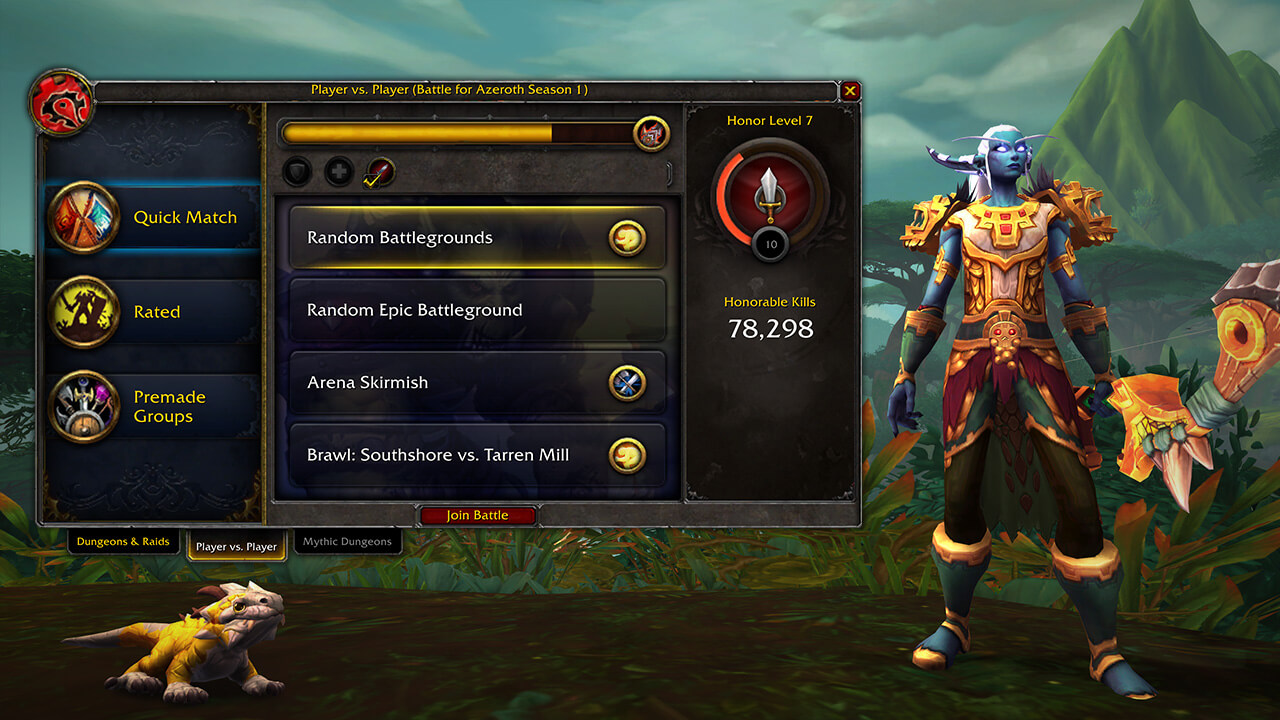
\includegraphics[width=0.75\textwidth]{Images/RewardSystems/WoWPvPRating.jpg}
    \caption{PvP player rating in World of Warcraft: Battle for Azeroth.}
    \label{fig:wow_player_rating}
    \vspace*{-0.5\baselineskip}
\end{figure}

\subsubsection{Experience Point Reward Systems}
Experience Points (XP) are utilized in the majority of games where players control developable avatars. XP are typically used to measure the players’ progress in the game, leveling up when a certain number of points is reached. The reward is classified as a “facility” type of reward, meaning a reward that increases the avatar skills at certain levels. XP are similar to score systems described above but differ in at least three ways:
\begin{itemize}
    \item XP are bound to specific avatars rather than the player itself.
    \item XP are rarely used for a ranking purpose.
    \item XP directly affects gameplay.
\end{itemize}

\subsubsection{Item Granting System Rewards}
This type of reward consists of in-game items that players or avatars can use. Item granting systems are often adopted in RPGs and MMORPGs to encourage exploration of the game world. Their primary purpose is to maintain players’ interest in-between intense battles, missions, or other exciting moments. Figure \ref{fig:wow_player_rating} illustrates a typical avatar in World of Warcraft wearing rewarded items.

\subsubsection{Resources}
Resources are in-game valuables collected and used in a way that affects the gameplay. The reward system is similar to an item granting system. Still, there is a significant difference between the two: Resources are mostly for practical game use, while items have a collecting and social value only. An example of resources is virtual wood and stone in Age of Empires Online. Figure \ref{fig:resources_age_of_empire} illustrates the tribute part of the game where players can donate resources to other players.

\begin{figure}[H]
    \centering
    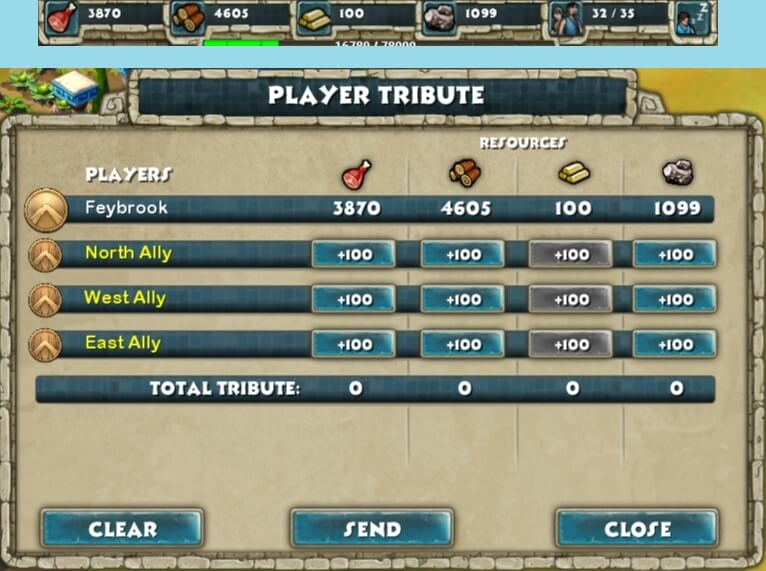
\includegraphics[width=0.75\textwidth]{Images/RewardSystems/AgeOfEmpireResources.jpg}
    \caption{Player tribute screen in Age of Empires Online.}
    \label{fig:resources_age_of_empire}
    \vspace*{-0.5\baselineskip}
\end{figure}

\subsubsection{Achievement Systems}
Achievement systems consist of titles bound to a user or avatar collected by completing clearly stated requirements. This type of reward encourages players to complete certain tasks, which may be more challenging than what they otherwise would have considered doing. Achievements can also be a way of improving the players’ urge to explore the game world. As an example, there are over a thousand different titles in World of Warcraft. Collecting these is publicly acknowledged by the community, consequently encouraging players to complete these tasks. Figure \ref{fig:wow_achievements} illustrates the achievement screen in World of Warcraft: Legion.

\begin{figure}[H]
    \centering
    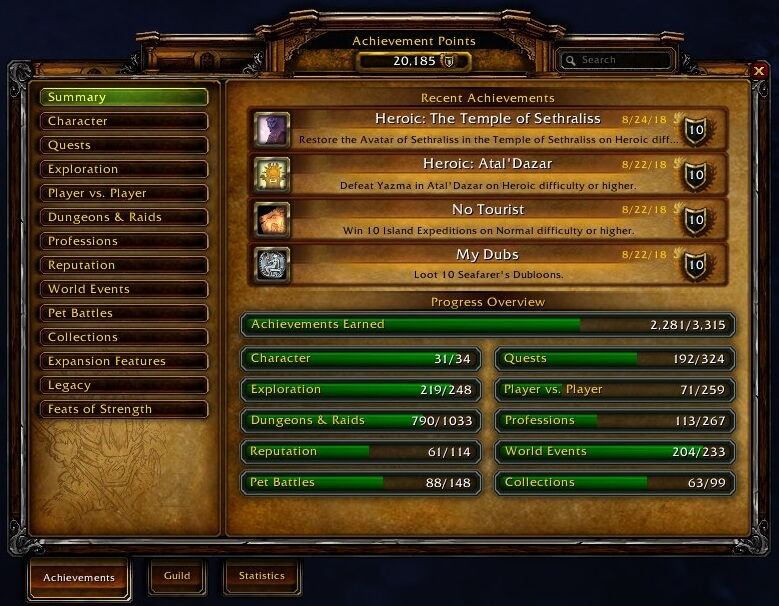
\includegraphics[width=0.7\textwidth]{Images/RewardSystems/WoWAchievements.jpg}
    \caption{Achievement screen from World of Warcraft: Legion.}
    \label{fig:wow_achievements}
    \vspace*{-0.5\baselineskip}
\end{figure}

\subsubsection{Feedback Messages}
Feedback messages provide instant feedback, an important element of flow \citep{sweetser_gameflow_2005}, to the player. The reward is not collectible, and thus, cannot be used as a player comparison or directly affect the gameplay. In Dance Dance Revolution, a message with the word “Perfect” appears every time you perform the correct dance move with precise timing, as seen in Figure \ref{fig:dance_dance_revolution_perfect}. This game element is a perfect example of a feedback message reward. The feedback can also be pictures, sound effects, or video clips.

\begin{figure}[H]
    \centering
    
\includegraphics[width=0.6\textwidth]{Images/RewardSystems/DanceDanceRevolution.jpg}
    \caption{Screenshot from Dance Dance Revolution.}
    \label{fig:dance_dance_revolution_perfect}
    \vspace*{-\baselineskip}
\end{figure}

\subsubsection{Plot Animations and Pictures}
Plot animations or pictures are used in games following notable events, such as completing a level or a mission. The purpose of this reward is to motivate players to continue advancing in the game. A famous plot animation is found in Super Mario Bros after completing a level. Figure \ref{fig:plot_animation_super_mario} illustrates this scene in New Super Mario Bros. U Deluxe.

\begin{figure}[H]
    \centering
    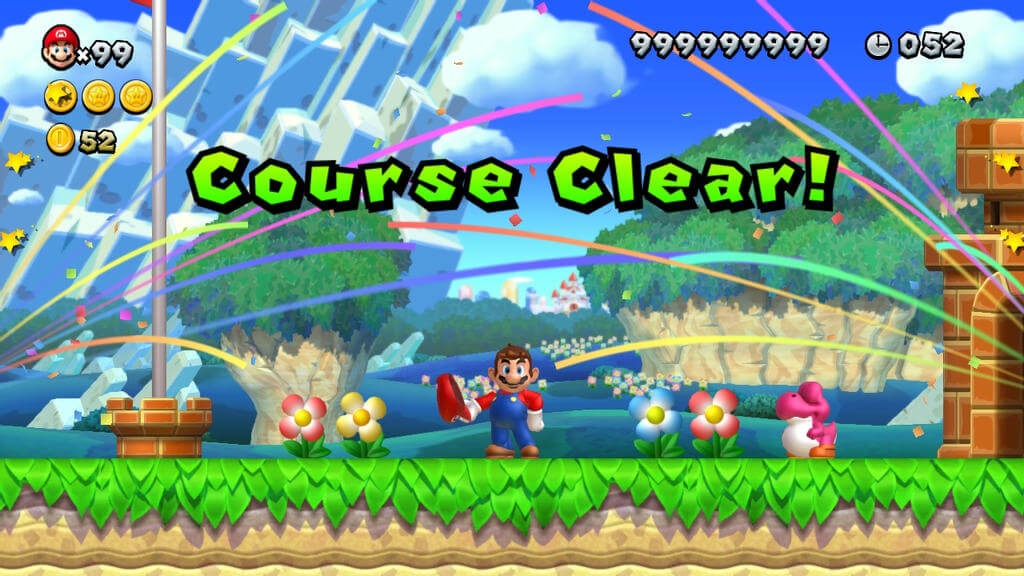
\includegraphics[width=0.75\textwidth]{Images/RewardSystems/SuperMarioBrosCourseClear.jpg}
    \caption{“Level completed” scene in New Super Mario Bros. U Deluxe.}
    \label{fig:plot_animation_super_mario}
    \vspace*{-0.5\baselineskip}
\end{figure}

\subsubsection{Unlocking Mechanisms}
The last reward type is unlocking mechanisms, which give players access to new game content when certain conditions, such as a new level or a special environment, are met. Unlocking mechanisms are hiding elements and awarding them to players as they progress in the game. The reward is substantial in regards to maintaining player curiosity. An example is found in World of Warcraft, where avatars must achieve certain levels before accessing higher-level environments.

\subsection{Design Consideration}
The article proposes seven reward system design considerations, which are directly relevant for us when we are going to develop our alternative game concept:

\textbf{Life Constraint}\\
Rewards must be available in a manner that fits the intended target group of the game. Hardcore gamers tend to spend more time playing; thus, the rewards should take longer to obtain. However, if the game is designed for casual gamers, the rewards should be accessible during shorter sessions.

\textbf{Create Autotelic Experiences}\\
The rewards should create intrinsically rewarding experiences. One way of doing this is to develop multi-level goals which will keep their engagement in the game. Players will then also learn and experience the pleasure of learning. 

\textbf{Balance}\\
An essential part of designing reward systems is to balance the time spent with the value of the reward. It is frustrating for players to feel like the rewards are never valuable enough. On the other hand, if the rewards are too valuable, the player might appreciate them less. 

\textbf{Uncertainty and Secrecy}\\
Uncertainty in rewards can create additional fun in games, but appropriate handling is essential. Not all reward types are suited for secrecy. For example, ammunition and life counts are typical rewards that are preferred to be exposed to the player. Other kinds of rewards such as treasures and quests may be hidden to introduce more fun. Hiding these elements encourages players to dive deeper into the game and spend more time exploring it. 

\textbf{Accumulated vs. Instant Feedback}\\
Accumulated rewards are important attributes for marking progress and comparing status between players. Accumulated feedback is appropriate for creating long term and social sense of achievement. Contrary, instant feedback provides responsiveness and an element of flow to the game.

\textbf{Social Purposes}\\
Game rewards enable social status that can be shared with others. Hard to get rewards, such as special items, distinguish advanced and casual players. These types of rewards also serve as a symbol to increase unity between skilled players.

\textbf{Physical World Activities}\\
Reward systems that support physical world activities impact the playing willingness. By being physically active, the guiltiness often associated with playing diminishes. An example is the physical world activities in Nintendo Wii, which changed the image of game playing.

\subsection{The Effect of Points and Audio in Kahoot!}
To conclude the topic of rewards systems in games, a concrete example of its importance will be briefly described. \citeauthor{wang_effect_2016} conducted a study in \citeyear{wang_effect_2016} looking at the effects of points and audio in the game-based learning system Kahoot!. Points as a reward system correspond to the “score systems” category, while audio classifies as “feedback messages,” according to the forms of rewards presented earlier in this chapter.  

The paper describes an experiment where Kahoot! was used as a learning method for teaching a lecture on software engineering. The students were divided into four groups using four different combinations of reward systems. The first group used Kahoot! as usual, with sound and audio. The second group played the game with audio but without points. The third group played Kahoot! without audio but with points, and the last group without audio and points. A questionnaire with statements related to concentration, engagement, enjoyment, learning, and motivation was filled out by the students after completing the lectures. 

The results from the study revealed notable differences in how the game was experienced in different groups. The effects of points and audio demonstrated a significant change in concentration, enjoyment, motivation, and engagement. The audio had a noticeable impact on classroom dynamics, but points also contributed to a more limited extent. An interesting observation was done in the group using Kahoot! where audio was removed, but points still present. The classroom was completely silent during the lecture, and students reported afterward that it felt more like a formal test than a game \citep{wang_effect_2016}.

The study illustrates the importance of reward systems in a game. Without points and audio in Kahoot! several of the students answered that they were less motivated and engaged.

\subsection{Summary}
In this chapter, a study of reward systems, including the eight different forms and seven design guidelines, has been introduced. In addition to this, a concrete example of the effects of reward systems in Kahoot! was presented. 

The content is highly relevant for our project and goal of developing an alternative game concept that has a socially beneficial effect. Especially in gamification concepts, reward systems are an essential tool for creating enjoyable games. In Part \ref{part:hover}, where our concept is presented, a concrete description of how reward systems are used will be given.
